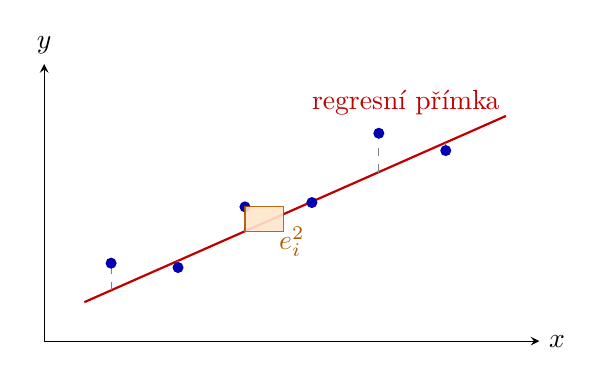
\begin{tikzpicture}[x=0.85cm,y=0.55cm,>=stealth]
    \draw[->] (0,0) -- (7.4,0) node[right] {$x$};
    \draw[->] (0,0) -- (0,6.4) node[above] {$y$};

    \draw[red!75!black,thick] (0.6,0.9) -- (6.9,5.2);

    \foreach \x/\y in {1/1.8,2/1.7,3/3.1,4/3.2,5/4.8,6/4.4}{
        \pgfmathsetmacro{\yh}{0.68*\x+0.49}
        \draw[dashed,gray] (\x,\yh) -- (\x,\y);
        \fill[blue!70!black] (\x,\y) circle (2pt);
    }

    \draw[fill=orange!20,draw=orange!70!black,opacity=0.9] (3,3.1) rectangle (3.57,2.53);
    \node[orange!70!black] at (3.7,2.3) {$e_i^2$};

    \node[red!75!black] at (5.4,5.5) {regresní přímka};
\end{tikzpicture}
